\documentclass[11pt]{article}
\usepackage[margin=1.0in]{geometry}
\usepackage[utf8]{inputenc}
\usepackage{graphicx}
\usepackage{hyperref}
%\usepackage{svg}
\usepackage{xcolor}
\usepackage{titlesec}
\titleformat{\section}[block]{\color{black}\large\bfseries\filcenter}{}{1em}{}
\titleformat{\subsection}[hang]{\bfseries}{}{1em}{}

%\usepackage{textcomp}
%\usepackage[dvipsnames]{xcolor}
%\usepackage{booktabs}
%\usepackage{soul}
\usepackage{subcaption}
%\captionsetup{compatibility=false}

%\usepackage{cleveref}
\setcounter{secnumdepth}{0}

\title{Towards a scalable and feedback-driven end-to-end movement and analysis framework of multimodal brain imaging data}
%\author{CS 452/652/752 Advanced Algorithms and Applications}
\date{}

\begin{document}

\maketitle
\clearpage
\section{Project Summary}
%What is multimodal imaging ?
\subsection{Overview}
%Noninvasive imaging techniques such as structural magnetic resonance imaging (S-MRI), diffusion MRI (D-MRI), functional MRI (F-MRI) and positron emission tomography (PET) play a key role in learning structural and functional properties of the brain. These different imaging modalities provide complementary information necessary to understand  the working dynamics of the brain.  However, effective processing, fusion, analysis, and visualization of multimodal data is challenging.  Most of the processing tasks associated with multimodal imaging are compute and data intensive. The other challenge stems from the presence of explicit variance and heteroginity across datasets, making it difficult to extract features and study a phenomena (disease).  Heteroginity in data arises due to variations in imaging resolutions or due to varying spatial-temporal dynamics. With our proposed collaborative research, we intend to address these fundamental challenges associated with multimodal imaging. We will begin by developing parallel algorithms and tools tailored towards scaling compute- and data- intensive processing tasks.  In particular, we will design a parallel data conversion tool that can efficiently transform data from one format to the other. We will also explore techniques to parallelize 3D volume segmentation. Finally, we propose to develop a machine-learning based performance model, that can provide valuable insight into data, help steer analysis in the right direction, and can also eventually  predict both patient outcome (clinical measures) and pathological progression based on a certain snapshot in space and time.

Noninvasive imaging techniques, such as structural magnetic resonance imaging (S-MRI), diffusion MRI (D-MRI), functional MRI (F-MRI) and positron emission tomography (PET), play a key role in learning structural and functional properties of the brain. These different imaging modalities provide complementary biomarkers necessary to understand the working dynamics of the brain. However, effective processing, fusion, analysis, and visualization of multimodal data are challenging. Most of the processing tasks associated with multimodal imaging are compute and data intensive. The other challenge stems from the presence of explicit variance and heterogeneity across datasets, making it difficult to extract features and study a phenomena (disease). Potential sources of heterogeneity in data include variations in imaging resolutions, spatial-temporal dynamics, disease phenotypes, and patient demographics. With our proposed collaborative research, we intend to address these fundamental challenges associated with multimodal imaging. We will begin by developing parallel algorithms and tools tailored towards scaling compute- and data- intensive processing tasks. In particular, we will design a parallel data conversion tool that can efficiently transform data from one format to the other. We will also explore techniques to parallelize 3D volume segmentation. Finally, we propose to develop a machine-learning based performance model that can provide valuable insight into data, help guide quantitative analysis workflow, and can eventually predict both patient outcome (clinical measures) and pathological progression based on a certain imaging snapshot in space and time.	

%Next we want to look at scaling 3D volume segmentation; various segmentation techniques of different accuracy and degree of complexity have been developed and reported in the literature. Atlas based segmentation, clustering, threshholding and machine learning based approaches are some of the popular techniques.
%we will target two of the most compute intensteps such as data format conversion and segmentation.
%We propose to address the computational and data management related challenges by developing parallel scalable tools and algorithms tailored towards processing steps such as data format conversion and segmentation. 

\subsection{Intellectual merit}
\begin{enumerate}
	\setlength\itemsep{-0.2em}
	\item Parallel data converter - why is it difficult and useful ?
	\item Parallel segmentation -  why is it difficult and useful ?
	\item Performance model -  why is it difficult and useful ?
\end{enumerate}

%In this paper we review the most popular methods commonly used for brain MRI segmentation. We highlight differences between them and discuss their capabilities, advantages, and limitations. To address the complexity and challenges of the brain MRI segmentation problem, we first introduce the basic concepts of image segmentation. Then, we explain differ


% at the heart of parallel segmentation lies parallelizing some of the existing clustering algorithm such as the K-means clustering. With the inclusion of these steps, we will end up with a scalable data movement framework, well suited for HPC platforms.


%Although many of these tasks are performed on HPC clusters, the tools used to perform these tasks are inherently serial in nature, and hence are unable to take advantage of the parallelism offered by the platform. There is also a considerable amount of manual intervention required to ensure that all the tasks are completed in the right order. For example, tasks such as data conversion (from one format to another) and 3D segmentation are performed serially using two different tools on the Cheaha supercomputer.




\subsection{Broader impacts}
TODO: With successful deployement of our research we will be able to transform the existing inefficient end-to-end data movement framwork to an efficient scalable feedback driven data movement and analysis framework, more.

%Previous studies aiming to explain biomarker variance typically focus on a single aspect of this heterogeneity: phenotypic heterogeneity at a coarse, typically late, disease stage or temporal heterogeneity in a broad population. However, the inability to disentangle the range of subtypes from the development and progression of each over time limits the biological insight these techniques can provide, as well as their utility for patient stratification. Constructing a comprehensive picture separating phenotypic and temporal heterogeneity, i.e. identifying distinct subtypes and characterising the development and progression of each, remains a major current challenge. However, such a picture would provide insights into underlying disease mechanisms, and enable accurate fine-grained patient stratification and prognostication, facilitating precision medicine in clinical trials and healthcare.


%It is becoming increasingly clear that combining multimodal brain imaging data provides more information for individual subjects by exploiting the rich multimodal information that exists. However, the number of studies that do true multimodal fusion (i.e., capitalizing on joint information among modalities) is still remarkably small given the known benefits.


%What are they used for ?
%What is the existing framework ?
%What are the deficiencies ?
%How is our proposed model going to help ?

%It is becoming increasingly clear that combining multimodal brain imaging data provides more information for individual subjects by exploiting the rich multimodal information that exists. However, the number of studies that do true multimodal fusion (i.e., capitalizing on joint information among modalities) is still remarkably small given the known benefits.

%In part, this is because multimodal studies require broader expertise in collecting, analyzing, and interpreting the results than do unimodal studies. In this article, we start by introducing the basic reasons why multimodal data fusion is important and what it can do and, importantly, how it can help us avoid wrong conclusions and help compensate for imperfect brain imaging studies. We also discuss the challenges that need to be confronted for such approaches to be more widely applied by the community. We then provide a review of the diverse studies that have used multimodal data fusion (primarily focused on psychosis) as well as provide an introduction to some of the existing analytic approaches. Finally, we discuss some up-and-coming approaches to multimodal fusion including deep learning and multimodal classification that show considerable promise.


%Currently, a large number of studies are collecting multimodal brain imaging data and information from the same participants. These imaging data types should be leveraged to extract the complementary information. For example, fMRI measures the hemodynamic response related to neural activity in the brain dynamically; sMRI enables us to estimate the tissue type for each voxel in the brain (gray matter [GM], white matter [WM], cerebrospinal fluid). Diffusion MRI can additionally provide information on the integrity of white matter tracts and structural connectivity. A key motivation for jointly analyzing multimodal data is to leverage the cross-information in the existing data, thereby revealing important relationships that cannot be detected by using a single modality.

%The heterogeneity of neurodegenerative diseases is a key confound to disease understanding and treatment development, as study cohorts typically include multiple phenotypes on distinct disease trajectories.



%Machine learning and pattern recognition algorithms have in the past years developed to become a working horse in brain imaging and the computational neurosciences, as they are instrumental for mining vast amounts of neural data of ever increasing measurement precision and detecting minuscule signals from an overwhelming noise floor. They provide the means to decode and characterize task relevant brain states and to distinguish them from non-informative brain signals.

%Existing framework for analyzing brain imaging data works

Describing the interdisciplinary research area to be explored and the innovative approach that will be undertaken, along with program objectives and goals (1 page maximum)\\


\begin{figure}
	\centering
	\begin{subfigure}{1\textwidth}
		\centering
		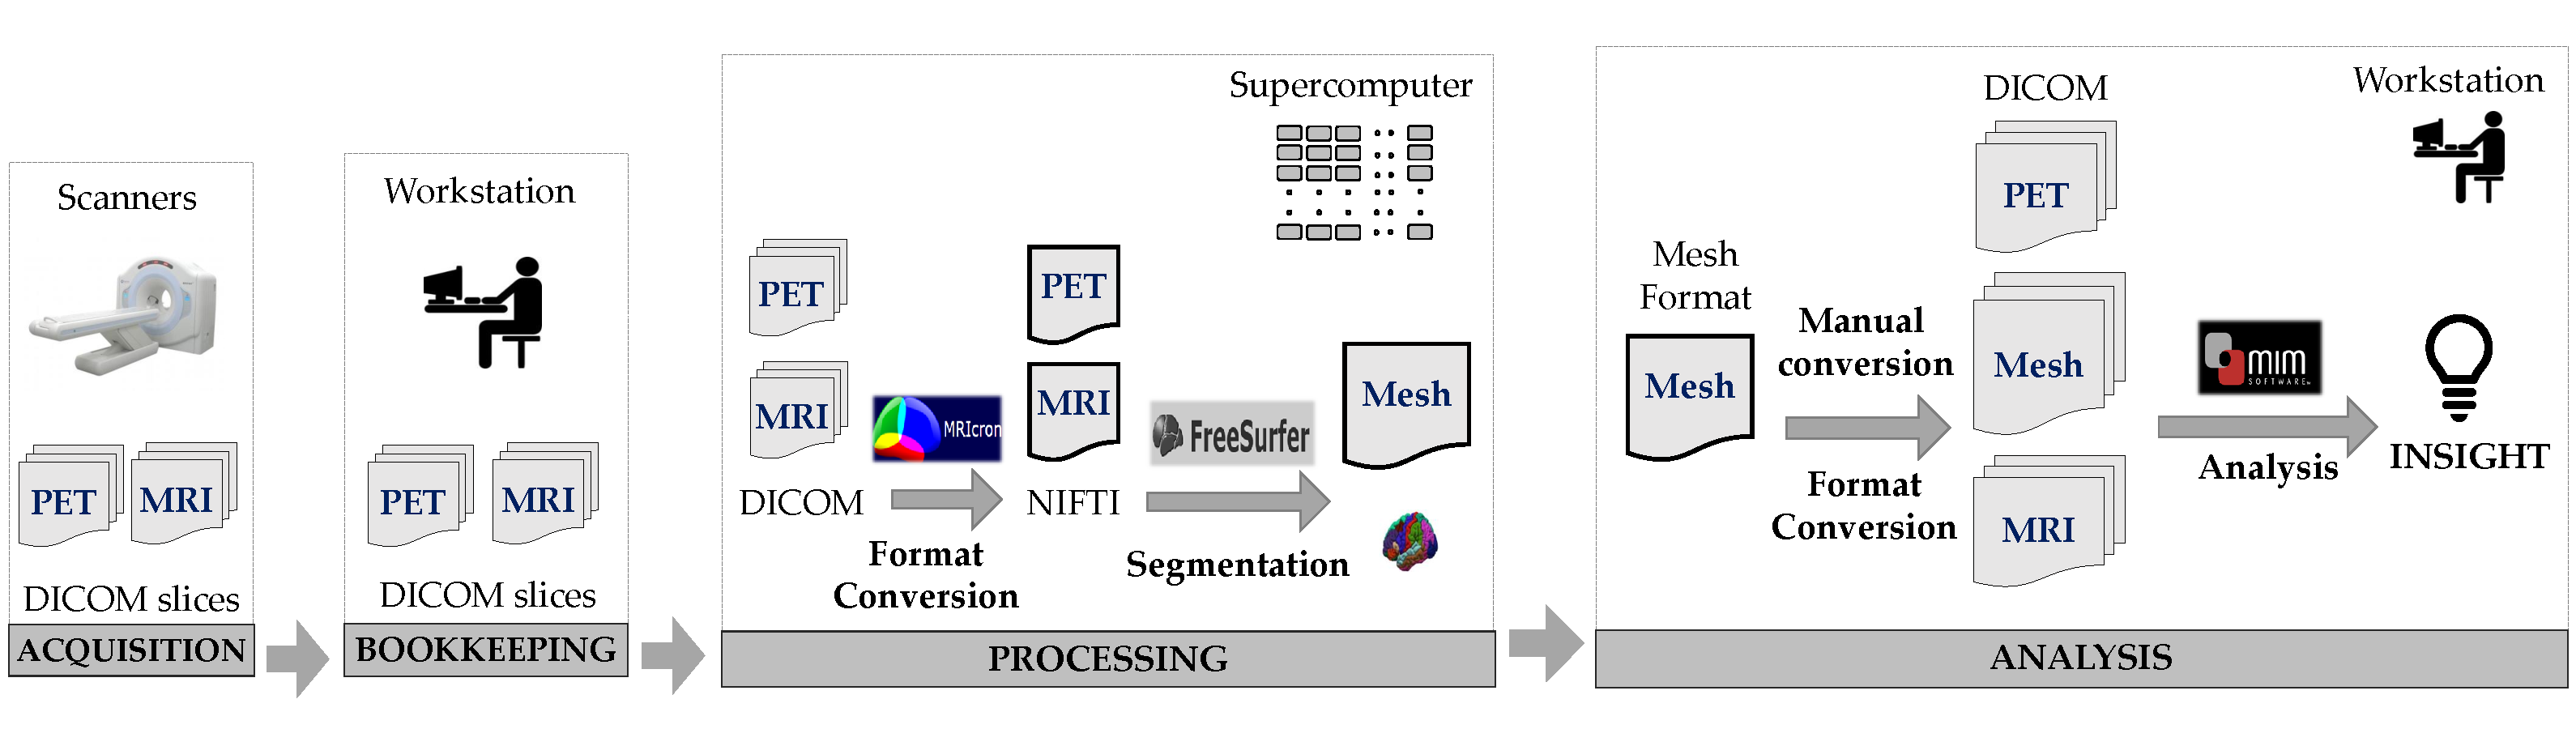
\includegraphics[width=\textwidth, height=4.5cm]{Existing.pdf}
	\end{subfigure}
	\caption {End-to-end movement and analysis framework of multimodal brain imaging data. The process begins with data being acquired from MRI and PET scanners, followed by pre-processing and analysis phases. The pre-processing phase includes the conversion of the data from the clinically used DICOM format to the analysis appropriate nifti format, followed by segmentation of the brain into regions such as the white matter, grey matter and XYZ. Once the pre-processing step finishes, the data is again converted back to the DICOM format which is then used to perform multimodal analyses using the MIM software framework.}
	\label{fig:theta_sens}
\end{figure}

\section{Team}
Dr Sidharth Kumar \\
Dr Jonathan Mcconathy \\
Fabio Raman \\
Grad student \\
Names, affiliations, and qualifications of the interdisciplinary research team (1 page maximum)

\section{Approach}

The task of extracting meaningful insights from multi-modal data (MRI and PET) involves several data transformation and processing steps;
example includes data format conversion, 3D segmentation, volume registration, kinetic modeling, uncertainity quantification and many other sophisticated analyses.
%Unfortunately, existing frameworks to facilitate end-to-end analysis (acqusuition from scanner to extracting meaning ful insight) of MRI/PET  data are inefficient, requiring constant human intervention.
Unfortunately, existing frameworks to facilitate these data transformation and processing steps does not scale well, and requires consistent human steering. 
Schematic diagram of exisiting end-to-end data movement and analysis framework is shown in ~\ref{}. As can be seen, data conversion and segmentation two of the computationally heavy steps are performed using serial tools MRICron and Freesurfer. We propose to develop tools that can transform data from one format to the other in parallel, making the process scalable and consequently take advanatage of the parallelism offered by a HPC platform. We also propose to develp parallel segmentation algorithms. Segmentation of 3D volume is challenging task.
In the last few decades, various segmentation techniques of different accuracy and degree of complexity have been developed and reported in the literature. Atlas based segmentation, clustering, threshholding and machine learning based approaches are some of the popular techniques used for segmentation. All these techniques are inherently serial, although there have been few work done in the past that has tried to perform segementaiton if 3D volumes in parallel, they did not see much speedups though, this was mainly because these tasks are bounded by communication. The existing HPC platforms such as the cheaha supercomputer has very low communication latency and also supports shared memory parallelism. We propose to develop parallel segmentation techniques, to 

The other major challenge associated with performing multimodal image analyses stems from the heteroginity and variance across datasets, making it difficult to track and identify distinctive features associated with a disease. For instance, neurodegenerative disorders, such as Alzheimer’s disease (AD), is biologically heterogeneous, producing high variance in vivo disease biomarkers, 
such as volumetric measurements from MRI imaging and kinetic modeling from PET imaging. Key contributors to this heterogeneity are that individuals belong to a range of disease subtypes (giving rise to phenotypic heterogeneity) and are at different stages of a dynamic disease process (producing temporal heterogeneity). This heteroginity makes it challenging to study a disease.
Previous work has mostly looked at a single aspect of this heterogeneity. Constructing a comprehensive picture separating spatial and temporal heterogeneity, continues to remain a major current challenge. However, such a picture would provide insights into underlying disease mechanisms, and enable accurate fine-grained patient stratification and prognostication, facilitating precision medicine in clinical trials and healthcare.

The task of extracting meaningful insights from multi-modal data (MRI and PET) involves several data transformation and processing steps;
example includes data format conversion, 3D segmentation, volume registration, kinetic modeling, uncertainity quantification and many other sophisticated analyses.
%Unfortunately, existing frameworks to facilitate end-to-end analysis (acqusuition from scanner to extracting meaning ful insight) of MRI/PET  data are inefficient, requiring constant human intervention.
Unfortunately, existing frameworks to facilitate these data transformation and processing steps does not scale well, and requires consistent human steering. 
Schematic diagram of exisiting end-to-end data movement and analysis framework is shown in ~\ref{}. As can be seen, data conversion and segmentation two of the computationally heavy steps are performed using serial tools MRICron and Freesurfer. We propose to develop tools that can transform data from one format to the other in parallel, making the process scalable and consequently take advanatage of the parallelism offered by a HPC platform. We also propose to develp parallel segmentation algorithms. Segmentation of 3D volume is challenging task.
In the last few decades, various segmentation techniques of different accuracy and degree of complexity have been developed and reported in the literature. Atlas based segmentation, clustering, threshholding and machine learning based approaches are some of the popular techniques used for segmentation. All these techniques are inherently serial, although there have been few work done in the past that has tried to perform segementaiton if 3D volumes in parallel, they did not see much speedups though, this was mainly because these tasks are bounded by communication. The existing HPC platforms such as the cheaha supercomputer has very low communication latency and also supports shared memory parallelism. We propose to develop parallel segmentation techniques, to 

The other major challenge associated with performing multimodal image analyses stems from the heteroginity and variance across datasets, making it difficult to track and identify distinctive features associated with a disease. For instance, neurodegenerative disorders, such as Alzheimer’s disease (AD), is biologically heterogeneous, producing high variance in vivo disease biomarkers, 
such as volumetric measurements from MRI imaging and kinetic modeling from PET imaging. Key contributors to this heterogeneity are that individuals belong to a range of disease subtypes (giving rise to phenotypic heterogeneity) and are at different stages of a dynamic disease process (producing temporal heterogeneity). This heteroginity makes it challenging to study a disease.
Previous work has mostly looked at a single aspect of this heterogeneity. Constructing a comprehensive picture separating spatial and temporal heterogeneity, continues to remain a major current challenge. However, such a picture would provide insights into underlying disease mechanisms, and enable accurate fine-grained patient stratification and prognostication, facilitating precision medicine in clinical trials and healthcare.

The task of extracting meaningful insights from multi-modal data (MRI and PET) involves several data transformation and processing steps;
example includes data format conversion, 3D segmentation, volume registration, kinetic modeling, uncertainity quantification and many other sophisticated analyses.
%Unfortunately, existing frameworks to facilitate end-to-end analysis (acqusuition from scanner to extracting meaning ful insight) of MRI/PET  data are inefficient, requiring constant human intervention.
Unfortunately, existing frameworks to facilitate these data transformation and processing steps does not scale well, and requires constant human intervention.
Although many of these tasks are performed on HPC clusters, the tools used to perform these tasks are inherently serial in nature, and hence are unable to take advantage of the parallelism offered by the platform. There is also a considerable amount of manual intervention required to ensure that all the tasks are completed in the right order.
For example, tasks such as data conversion (from one format to another) and 3D segmentation are performed serially using two different tools on the Cheaha supercomputer.


Besides being inefficient, the existing data analysis pipeline is also very brute force in nature. 
For example, finding the efficacy of segmentation process and time-activity curves rely on visual inspection.
Segmented output and time-activity both these tasks also vary across individuals. Besides different PET tracers have varying time activity behavior.
Segmentation continues to be one of the challenging problem in the field of image processing. Direction that is being explored more rigorously is 
to combine multimodal brain imaging data that provides more information for individual subjects by exploiting the rich multimodal information.


%Other major challenge faced by clinicians is with respect to the actual analysis of the imaging data.
%It is becoming increasingly clear that combining multimodal brain imaging data provides more information for
%individual subjects by exploiting the rich multimodal information that exists. However, the number of studies that do
%true multimodal fusion (i.e., capitalizing on joint information among modalities) is still remarkably small given the
%known benefits. In part, this is because multimodal studies require broader expertise in collecting, analyzing, and
%interpreting the results than do unimodal studies. In this article, we start by introducing the basic reasons why
%multimodal data fusion is important and what it can do and, importantly, how it can help us avoid wrong conclusions
%and help compensate for imperfect brain imaging studies.

Finally, we discuss some up-and-coming approaches to multimodal fusion
including deep learning and multimodal classification that show considerable promise.


\subsection{Existing pipeline}
PET and MRI data acquired from scanners initially resides at the MIM~\cite{} cloud server. Although the spatial resolution of the datasets are small ($512 \times 512 \times 512 = 1 GB$), the scans are performed at high temporal frequencies, resulting in large volumes of data. For example, one PET scan can easily have upto 8000 or more time-steps, which for a $512^3$ resolution scan is approximately $8$ TB. Existing movement and processing pipeline of these images does not scale, is inefficient and requires a lot of manual intervention. The data is first copied to a local workstation, where a user tags and makes a local record of all the datasets. Next, the dataset is copied to the Cheaha supercomputer ~\cite{bibid}. The first step is the conversion of data from the clinically used DICOM~\cite{} format to the analysis appropriate nifti ~\cite{} format. Nifti is the defacto format when comes to performing analysis and processing related task. In nifti, data exists in just one single file, as opposed to Dicom, where the 3D volume resides in n Z order 2D slices. This step of converting Dicom to nifti is performed sing the open-source software Mricron~\cite{}. Mricron suffers from the following three pitfalls
\begin{enumerate}
	\setlength\itemsep{-0.2em}
	\item Allows serial execution, hence, failing to use the underlying parallelism offered by the Cheaha supercomputer
	\item Conversion is lossy w.r.t to the metadata (patients records, and slice info)
	\item Does not support conversion from Nifti back to the DICOM format.
\end{enumerate}

The next step is 3D segmentation of the brain MRI dataset. Currently, Freesurfer~\cite{}, another freely available software is used for segmentation. The segmentation of the brain data leads to clustering of all voxels into 40 different regions of the brain ~\cite{}. For AD, a scientist is typically only interested in 3 regions of the brain, the grey matter, the white matter and Dome fluid. 3D segmentation is very compute intensive and ofter requires several hours for completion. Freesurfer, uses atlas based~\cite{} techniques to perform segmentation, but similar to MRIcron, it also does not support parallel execution. Freesurfer, therefore does not take advantage of the parallelism offered by the Cheeaha supercomputer. User, most of the time, run several batch jobs in parallel, each corresponding to segmentation of one 3D volume.

The segmented mesh is copied back to the local workstation. MIM is used for the final analysis of the brain scans. MIM is a robust, a very popular closed source software tool that is used for kinds of analysis tasks. Usually MRI and PET scans are both usedat once to make better sense of what is happening. Both MRI and PET data needs to be registered to the segmented mesh to associate context to the scans. MIM is a clinically approved software framework,and hence only uses the clinically approved DICOM data format. Therefore, a user has to first convert the mesh data innifti format generated from freesurfer back to the DICOM format.Unfortunately, MRIcron does not support this conversion. A user typically has to use some third party tool like freeslicer that loads the nifti data, manually enters metadata and then convert the data into 2D dicom slices. This process is a wasteful of both the user's time as well as compute resources.



% Freesurfer, similar to Mricron does not allow for parallel execution, The 3D MRI data existing in the nifti format, is then 



Data sources: X, Y, Z \\
What does PET data have ? \\
What does MRI have ? \\
1. Difficult to identify regions in scan that ? \\
2. Difficult to track these regions over time ? \\
3. Time-activity curve extracted from PET data, varies across individuals, difficult to correlate time activity with the time-steps. \\


Methodology, data to be collected, and how different disciplines will interact to achieve program goals

%\begin{figure}
%	\centering
%	\begin{subfigure}{1\textwidth}
%		\centering
%		\includegraphics[width=\linewidth]{Existing_workflow.pdf}
%		\caption{Mira, 32K particles}
%	\end{subfigure}
%	\hspace{-0.25cm}
%	\begin{subfigure}{1\textwidth}
%		\centering
%		\includegraphics[width=\linewidth]{Proposed_workflow.pdf}
%		\caption{Mira, 64K particles}
%	\end{subfigure}
%	\caption {Data movement framework}
%	\label{fig:mira_sens}
%	\label{fig:theta_sens}
%	%\vspace{-.1in}
%	\vspace{-1em}
%\end{figure}

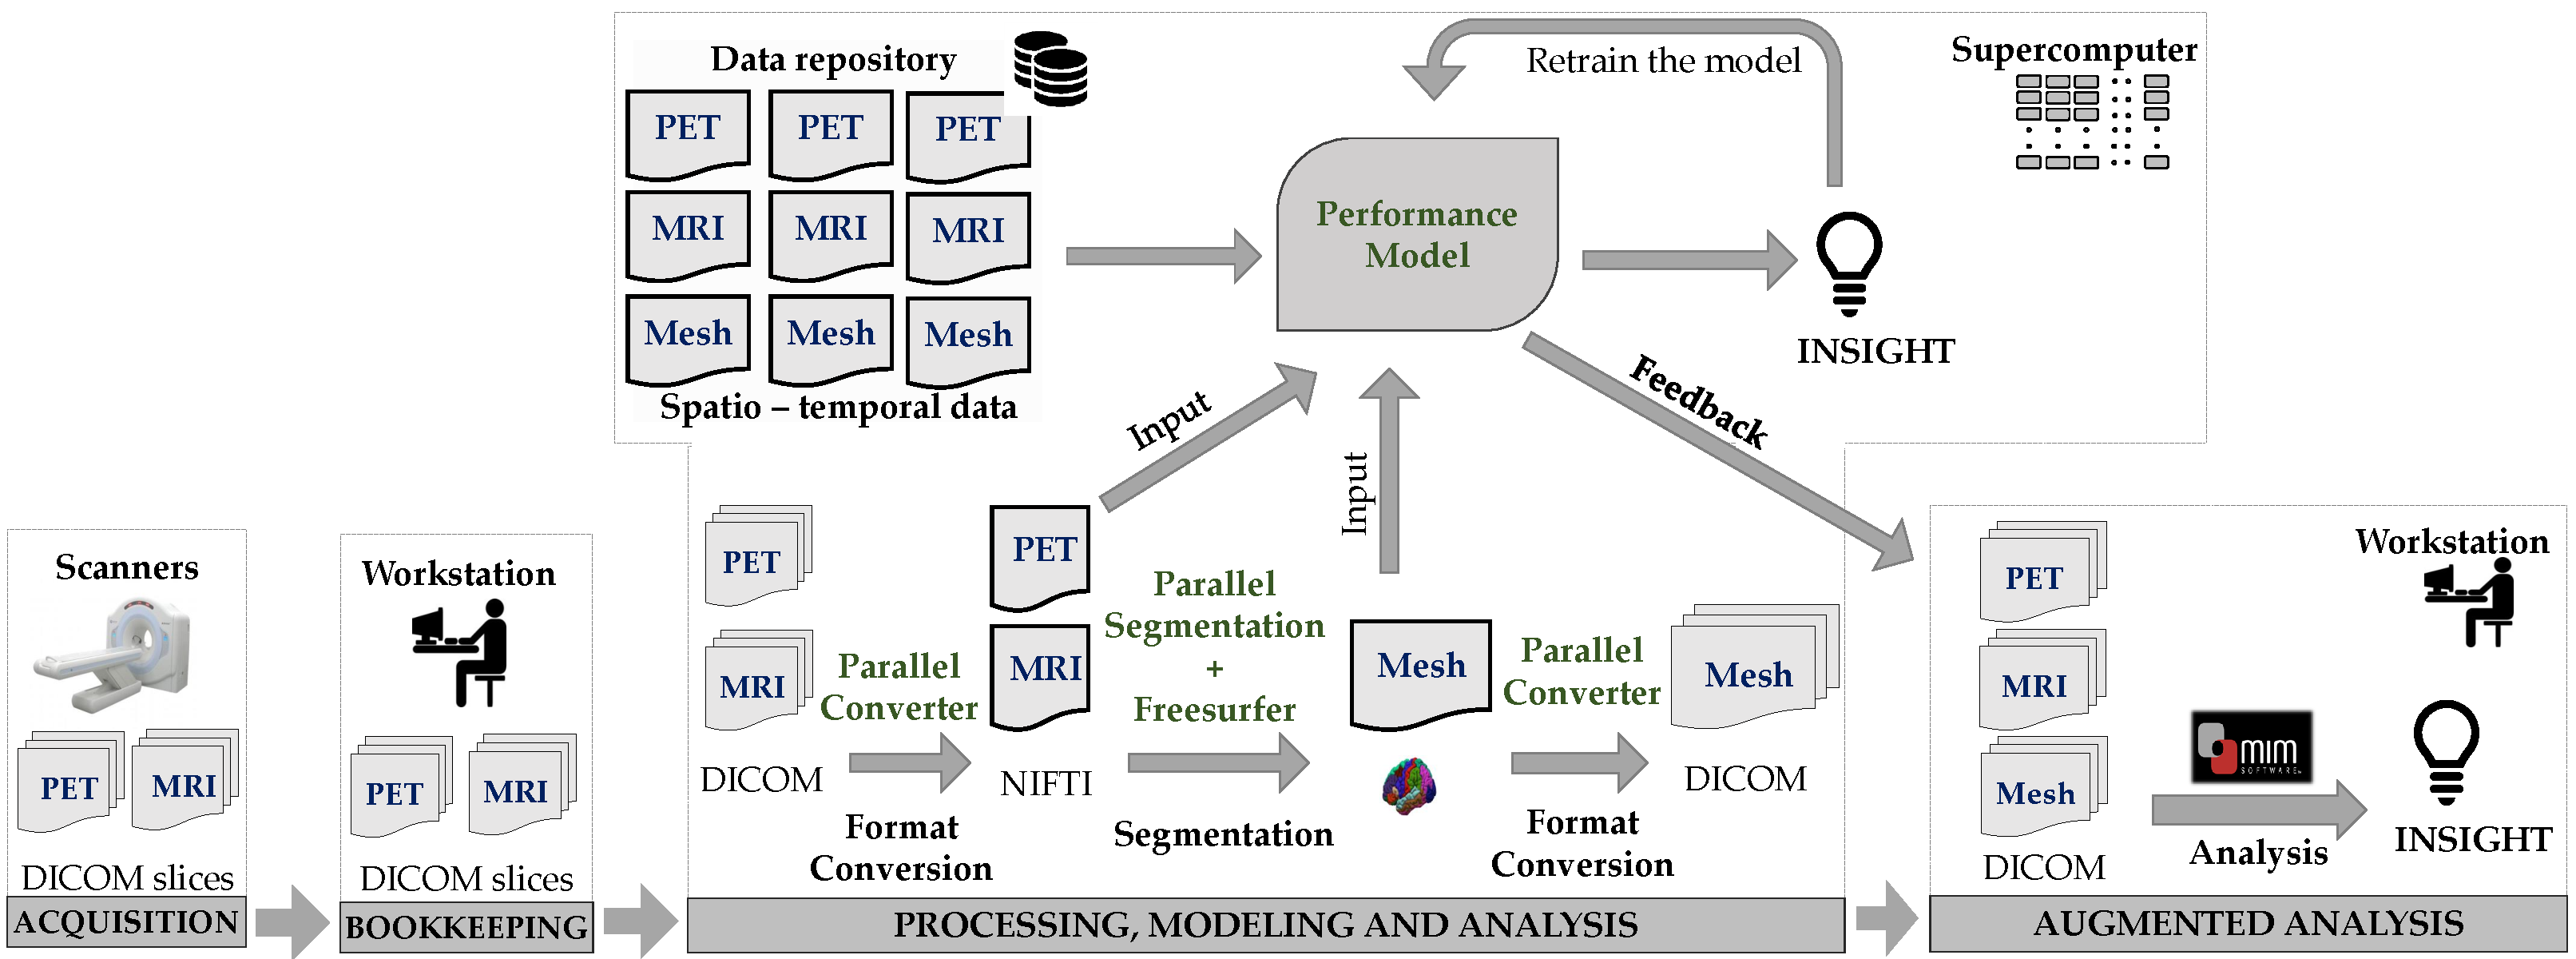
\includegraphics[width=1\textwidth, height=7cm]{Proposed.pdf}\\

\section{Anticipated Outcomes}

\subsection{Deliverables}

Parallel data converter \\
Parallel segmentation \\
Deep-learning based performance model \\

\subsection{Future direction}
This research is going to lay foundation for a long term collaboration between the computer science and the radiology department. We are trying to solve some of the very basic problems faced in the field of imaging. The ultimate goal is to develop a suit of techniques that can be universally adopted by imaging experts from fields such as radiology, X, Y, Z. To this end, we want to revam the existing inefficient manual data movement and analysis framework to an fully automiatic feedback driven framework that can not only aid clinicians make better sense of the data. This research will enable the first step towards building a long lasting collaboration.

With this research we are targeting to solve the most fundamental problem

Scholarly activities and technological impacts that are
expected at the successful completion of the project. How the interdisciplinary
team will proceed after the initial seed funding to sustain the project and seek
extramural support. Also, describe the commercialization potential for this
interdisciplinary project if applicable. The prospect of follow-on extramural
support for the project will be an important review criterion (2 pages maximum).

\section{Budget and budget justification}
The budget and budget justification should cover a support period of one year (2 pages maximum). The budgeting of PI’s and co-PI’s salaries or release time is discouraged.  

\end{document}
